\documentclass[12pt,a4paper]{article}

\usepackage[UTF8]{ctex}
\usepackage{geometry}
\usepackage{graphicx}
\usepackage{booktabs}
\usepackage{hyperref}
\usepackage{setspace}
\usepackage{float}
\usepackage{caption}
\usepackage{array}
\usepackage{longtable}

\geometry{left=2.5cm,right=2.5cm,top=2.5cm,bottom=2.5cm}
\onehalfspacing
\sloppy
\graphicspath{{figures/}}
\hypersetup{colorlinks=true,linkcolor=black,urlcolor=blue,citecolor=black}

\title{From Fusion to Switching: Intercultural Experience Along a Macau Route}
\author{UCUG1600 Cross-Cultural Communication Final Group Report\\
Group members, in contribution order: TBC}
\date{8 May 2026}

\begin{document}
\renewcommand{\abstractname}{Abstract}
\renewcommand{\figurename}{Figure}
\renewcommand{\tablename}{Table}
\maketitle

\begin{abstract}
Macau is often called a city of ``Chinese-Western fusion.'' The label fits part of the reality. Bilingual street signs, Portuguese-style architecture, and World Heritage streets are there on the ground. Yet a one-day field trip showed us more than fusion can account for. Based on photos, videos, and route notes collected in April 2026, this report follows a route from the border through commercial streets and the Ruins of St.\ Paul's to the Venetian in Cotai. It examines how five kinds of urban space place the observer in different cultural positions: entrant at the border, consumer in commercial streets, viewer in the historic area, participant in themed entertainment, and passenger on the bus. The report introduces ``cultural role switching'' to describe these shifts and argues that Macau's intercultural character does not stay fixed in any one place but changes with movement along the route. This finding supplements the fusion label by showing that spatial movement itself shapes intercultural understanding.
\end{abstract}

\section{Introduction}

The first thing we noticed at the Macau border was the sound. Escalators hummed, announcements echoed in three languages, and hundreds of people shuffled forward in queues without talking much. Nobody was looking at heritage architecture. They were reading overhead signs, holding documents, trying to figure out which line to join. This was Macau too, even though no tourist brochure describes it.

Macau is labelled a city of ``Chinese-Western fusion,'' and the label is partly right. The UNESCO-listed Historic Centre of Macao does show long-term exchange between China and the West in architecture, religion, and urban technology (UNESCO World Heritage Centre, n.d.). Chinese-Portuguese street names and Catholic church facades are real and visible. The trouble is that ``fusion'' suggests something settled and blended, while what we experienced on the ground kept shifting. Near the Ruins of St. Paul's, food stalls and souvenir crowds pulled us into buying before we ever reached the stone facade. In Cotai, the Venetian's painted sky and an NBA shooting game folded European imagery and American sports into the same shopping route. On the bus between stops, the city appeared frame by frame through the window.

This report asks a straightforward question: how do Macau's urban spaces change what observers do and notice as they move through them? We use ``cultural role switching'' to describe how different spaces place the observer in different positions, entrant at the border, consumer on the food streets, viewer in the historic area, participant in Cotai, passenger on the bus. These shifts connect to the course themes of self and other, cultural sensitivity, and verbal and non-verbal communication. We let the field materials lead, fitting each site to what we observed, not to a preset concept.

The analysis is limited to public spaces along one field trip route. We did not conduct interviews, so we do not speak for Macau residents, tourists, or workers. What follows introduces the concepts and methods, walks through five kinds of space along the route, and discusses what this approach adds to understanding intercultural communication in Macau.

\section{Conceptual framework and literature review}

This report draws on four areas of literature: routes and the positioned observer, tourism and staged experience, linguistic landscape and non-verbal communication, and Macau's own heritage and language politics. These four areas give us tools to read what we saw without attaching a concept to every site.

\subsection{Space, route and the positioned observer}

Urban space shapes how people enter, look, pause, and make sense of a place. Lefebvre's (1991) idea of the production of space treats space as something made through social relations, institutional arrangements, and everyday practices. Along our Macau route, border corridors, heritage steps, and bus interiors each arranged people's movements in different ways. de Certeau (1984) reads walking as a daily practice through which people use and interpret the city. For us, the route was part of the analysis itself. Macau's cultural differences became visible precisely through the transitions between spaces.

Pink's (2009) work on sensory ethnography pushes in the same direction. Field observation that relies only on images misses a lot. Crowd density, noise, movement speed, and physical tiredness all shaped what we noticed. Some of the sharpest observations came during transitions, the moments between one space and the next, rather than at the planned stops. Including them keeps this report from becoming a checklist of tourist sites.

\subsection{Tourism, authenticity and staged experience}

Tourism spaces often decide in advance what visitors see and how they photograph. MacCannell's (1973) concept of staged authenticity explains how tourism settings arrange a version of the ``real'' for visitors to consume. Wang (1999) pushes authenticity further: even when an object is not historically original, the feeling of participation can still produce a lived experience. Urry and Larsen's (2011) tourist gaze shows that tourist viewing is shaped by attractions, photo positions, and social expectations, while Edensor (2000) notes that photographing, shopping, and queuing are part of how tourism spaces are completed by visitors.

These ideas help separate the Ruins of St. Paul's from the Venetian. Both use European symbols. Both attract photography. The viewing practice is different. The Ruins of St. Paul's depends on historical remains and World Heritage status. The Venetian depends on reproduced facades, indoor sky ceilings, and retail streets designed for immersion. One is heritage viewing, the other is immersive consumption. Macau is unusual because both can appear on the same route in a single afternoon.

\subsection{Linguistic landscape and non-verbal communication}

Intercultural communication happens outside conversation too. Landry and Bourhis (1997) define the linguistic landscape as the visibility of languages in public space: street names, signs, advertisements, shopfronts. Scollon and Scollon's (2003) geosemiotics asks us to read signs through their location, direction, and material, not just their words. In Macau, Chinese-Portuguese street signs, hotel wayfinding systems, and NBA product labels all count as public signs worth reading.

Non-verbal communication runs through the same spaces. Hall (1959) describes space itself as a silent language, an idea that fits the border queues, the quiet of a church interior, and the noise of a shooting game. UCUG1600 places weight on both verbal and non-verbal communication. Macau is a good case for this: some cultural information is written on signs, while the rest is carried by movement, lighting, and crowding.

\subsection{Macau studies and course lens}

Macau studies brings these wider theories back to a specific place. Chung (2009) links Macau's heritage conservation with urban development and identity narratives. Chu (2015) studies spectacular urban space in Macau, showing how Cotai hotels reshape the urban imagination through visual scale and themed architecture. Yan (2019) examines language choices in Macau's public space and connects them to identity and power. Ma and Mu (2023) show that multilingual signs in Macau are arranged according to place function and target readers.

The pattern across these studies is clear: ``Chinese-Western fusion'' describes part of Macau but not all of it. A more useful question is how different spaces arrange the relationship between observers and cultural signs, a question that connects with the course themes of self and other, cultural sensitivity, and intercultural storytelling. We ask how spaces work in their settings, not whether they are ``real'' or ``fake.''

\section{Methodology}

\subsection{Field site and route}

The materials come from a Macau field trip during the course fieldwork period in April 2026. Our group entered Macau's public spaces as both students and visitors. The route ran roughly: border and immigration space $\rightarrow$ transport area and road views outside the border $\rightarrow$ historic commercial streets $\rightarrow$ the Ruins of St. Paul's, church spaces, sacred art spaces, and Mount Fortress $\rightarrow$ bus and road transitions $\rightarrow$ Cotai hotel complexes, the Venetian, and NBA-themed space $\rightarrow$ return transport. Transit spaces are included in the Findings because movement kept changing the observer's position. They are not empty time between destinations.

\subsection{Data collection methods}

The group recorded crowds, movement routes, signs, architecture, and interactive practices. Photos and videos preserved scenes such as border direction signs, commercial street crowds, bilingual street signs, the Venetian ceiling, the NBA shooting area, and vehicle window views. The route itself was also treated as material, since it showed how one place shifted into another. Field notes also covered sound levels, light conditions, and physical tiredness. After organising the materials, the group had about 69 logical media items, including photos, videos, and selected frames extracted from videos. Images in the report were chosen because they supported the argument and did not foreground identifiable individuals.

\subsection{Scope, ethics and AI use}

The field trip did not include formal interviews, so the report cannot represent the subjective views of Macau residents, tourists, shopkeepers, or workers. The analysis is limited to observable elements in public space: languages, buildings, sound, movement routes, crowds, and consumption signs. When images include crowds, they are used only as evidence of how public space is used, such as tourist viewing or transport density. The report does not analyse identifiable individuals.

Generative AI assisted with early theme exploration and keyword suggestions. The group selected the research question, chose the materials, and built the argument. All field observations come from the actual trip.

\section{Findings}

This section follows the field trip route in order. Commercial streets are discussed before the historic area because, in our experience, visitors usually passed through food stalls and crowds before reaching the Ruins of St. Paul's. Transit is treated separately because buses and bridges changed the angle of observation and made different versions of Macau appear in motion.

\subsection{Border Macau}

The first Macau we met that day was made of escalators, direction signs, and transport connections. Nobody saw the Ruins of St. Paul's from the immigration hall. Before entering the city proper, we were already reading signs, following crowds, and switching between transport modes. Intercultural experience started here, but it started as managed movement.

\begin{figure}[H]
  \centering
  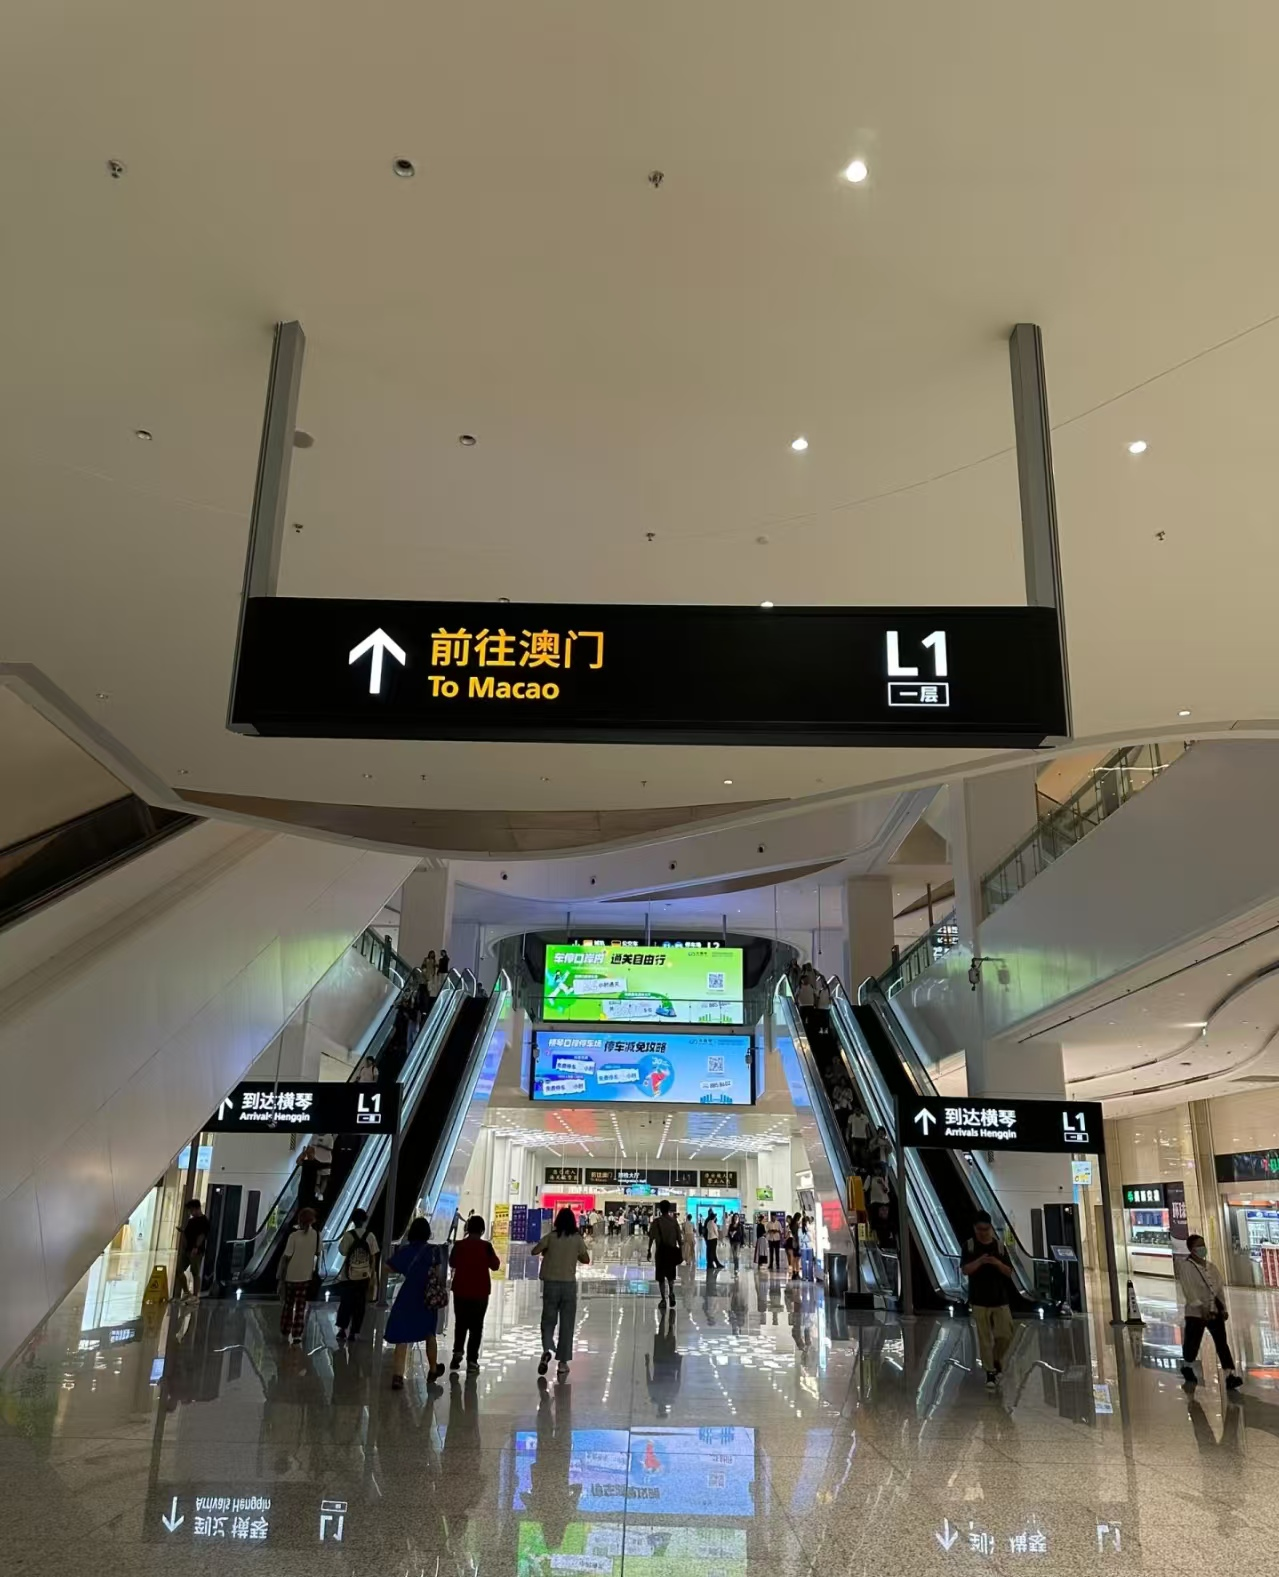
\includegraphics[width=0.82\linewidth]{fig01_border_sign.jpg}
  \caption{Transport and wayfinding space on the way to Macau. Direction signs, escalators, and transport nodes appear before tourist sites and first set the body's direction of movement.}
\end{figure}

Communication at the border did not rely on face-to-face dialogue. Direction signs, escalators, and corridors told people where to go. Hall's (1959) idea of space as a silent language fits here: rules were rarely explained at length, but bodies still moved along certain paths without asking questions. Macau at this stage felt less like a cultural scene to look at and more like a system to pass through.

\subsection{Commercial streets}

After leaving the border and transport space, the route entered commercial streets near the Ruins of St. Paul's. This was no quiet entrance into history. Food stalls hit first. The smell of egg tarts and beef jerky came before any stone facade. Souvenir shops, dense signs, and multilingual shop names pulled visitors into a tourist version of Macau before the heritage site had even appeared.

\begin{figure}[H]
  \centering
  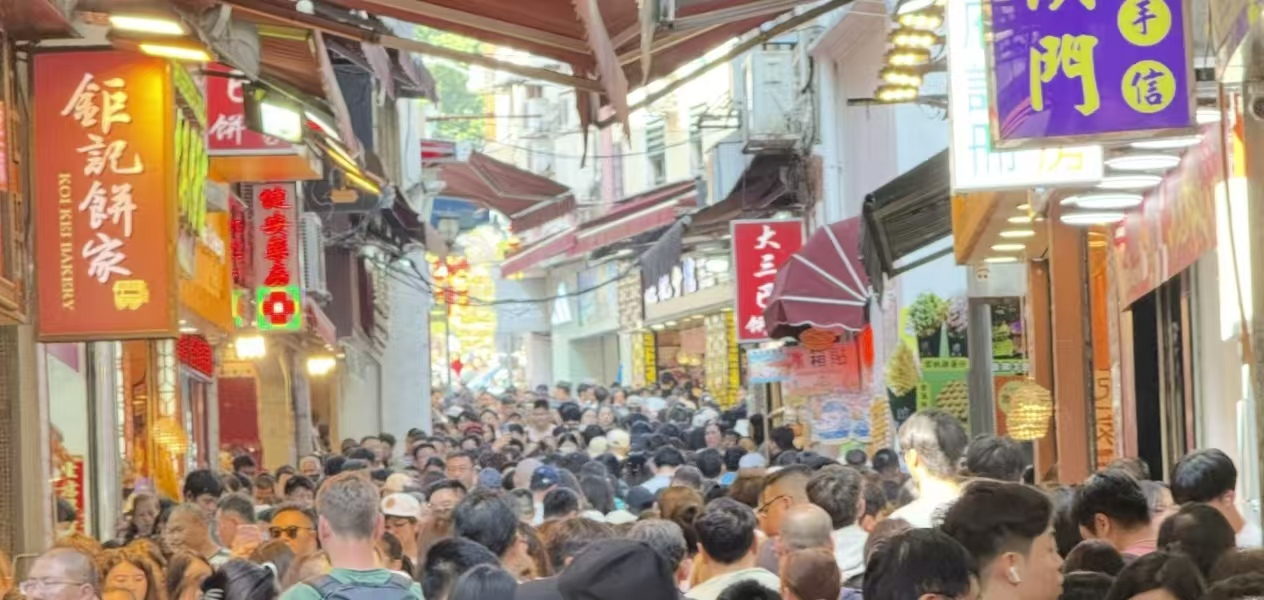
\includegraphics[width=0.82\linewidth]{fig02_commercial_crowd.jpg}
  \caption{Dense crowds in a commercial street near the Ruins of St. Paul's. The route to the heritage landmark first passes shops, signs, and crowded tourist movement.}
\end{figure}

Languages on the commercial street had a clear division of labour. Chinese carried the everyday commercial talk between shopkeepers and customers. English helped tourists identify goods and services. Portuguese, often smaller on the sign, marked Macau's historical identity visually. Landry and Bourhis (1997) remind us that visible language in public space shapes how people understand place identity. In these streets, multilingual signs worked alongside product displays and tasting stands, not in isolation.

\begin{figure}[H]
  \centering
  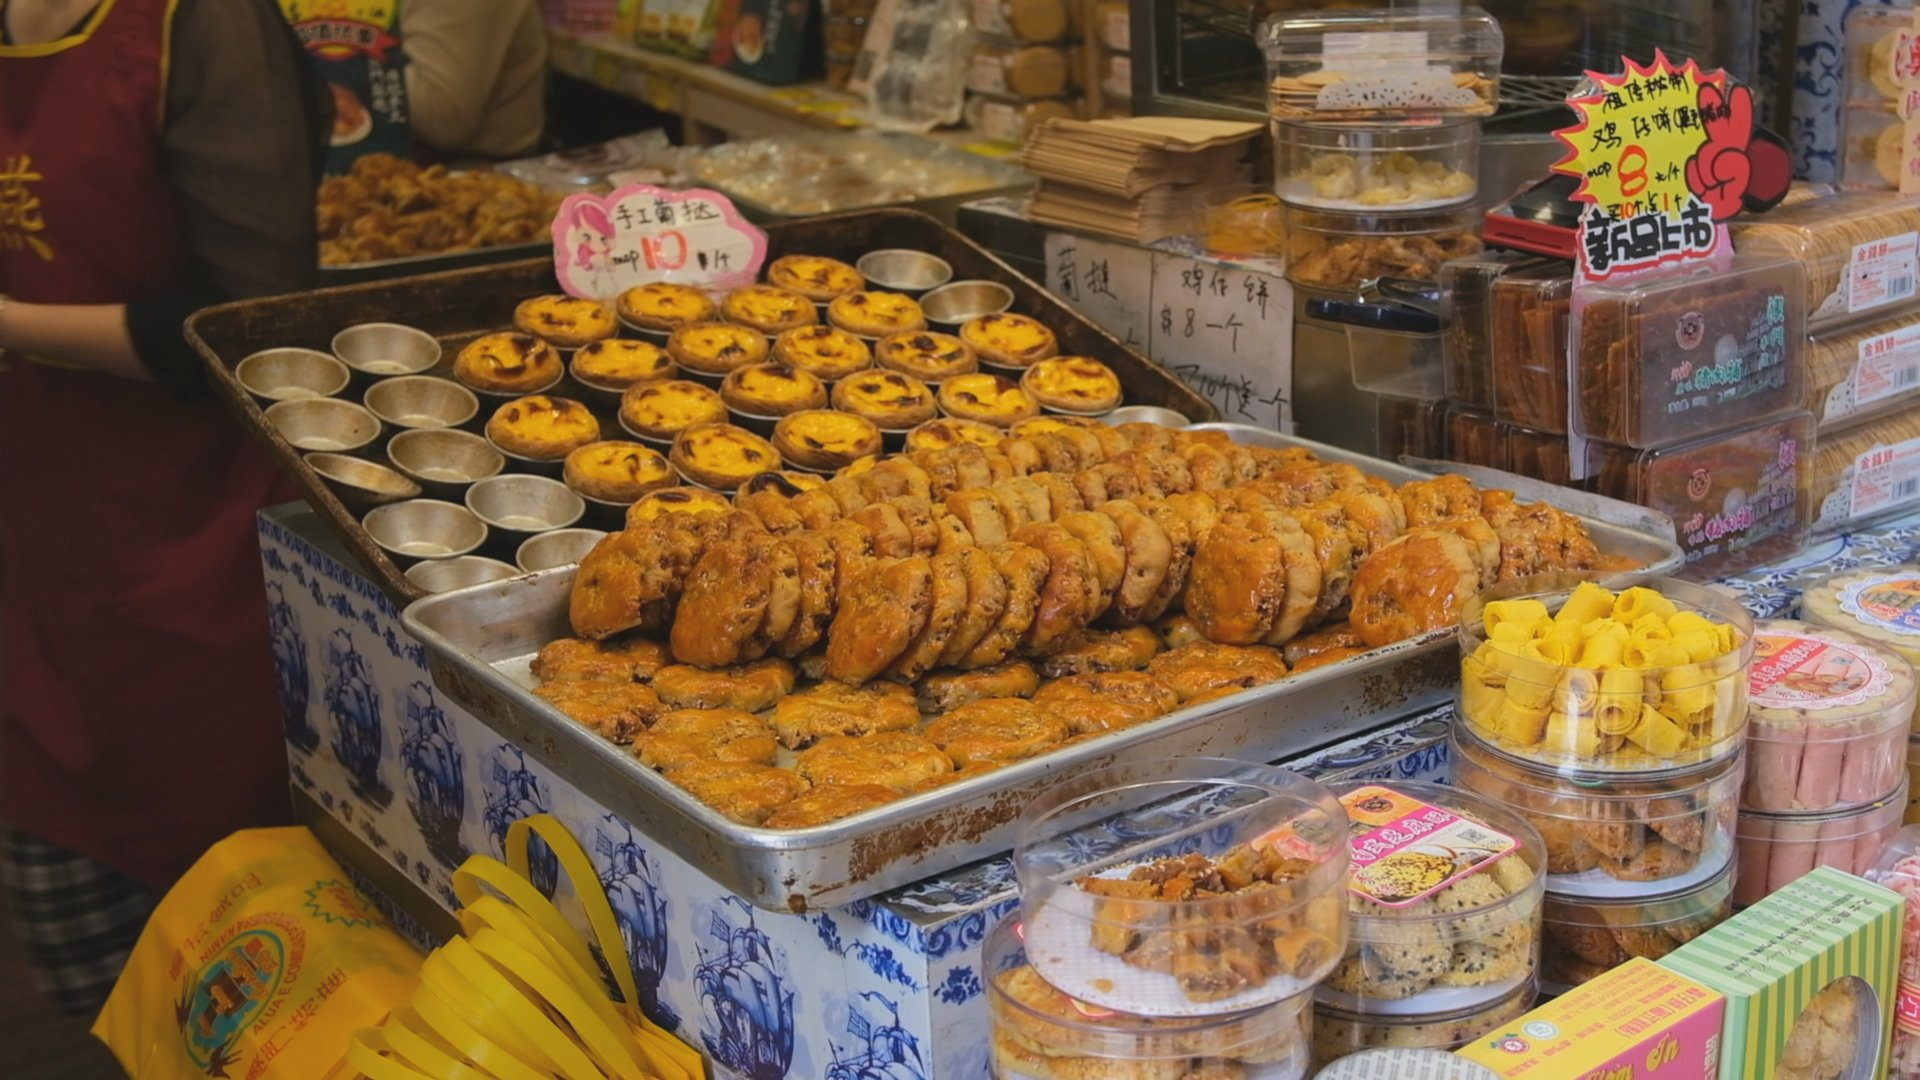
\includegraphics[width=0.82\linewidth]{fig03_food_street.png}
  \caption{Street bakery and snack stall. Taste, purchase, and brief stops let visitors enter the commercialised historic district through the body and senses.}
\end{figure}

In this street space, the observer's clearest role was consumer. People looked at signs, bought snacks, and followed the crowd toward the Ruins of St. Paul's. Commerce packaged the heritage landmark into a tourist experience that was easy to enter and hard to skip. For us, Macau's history arrived through taste and crowd movement before any textbook version.

\subsection{Historic Macau}

After the commercial streets, the pace changed. The historic area around the Ruins of St. Paul's, church spaces, and Mount Fortress required a different kind of attention. You had to slow down, look up at facades, read street signs, and move through slopes and stone walls. The history was there, but you had to walk into it.

\begin{figure}[H]
  \centering
  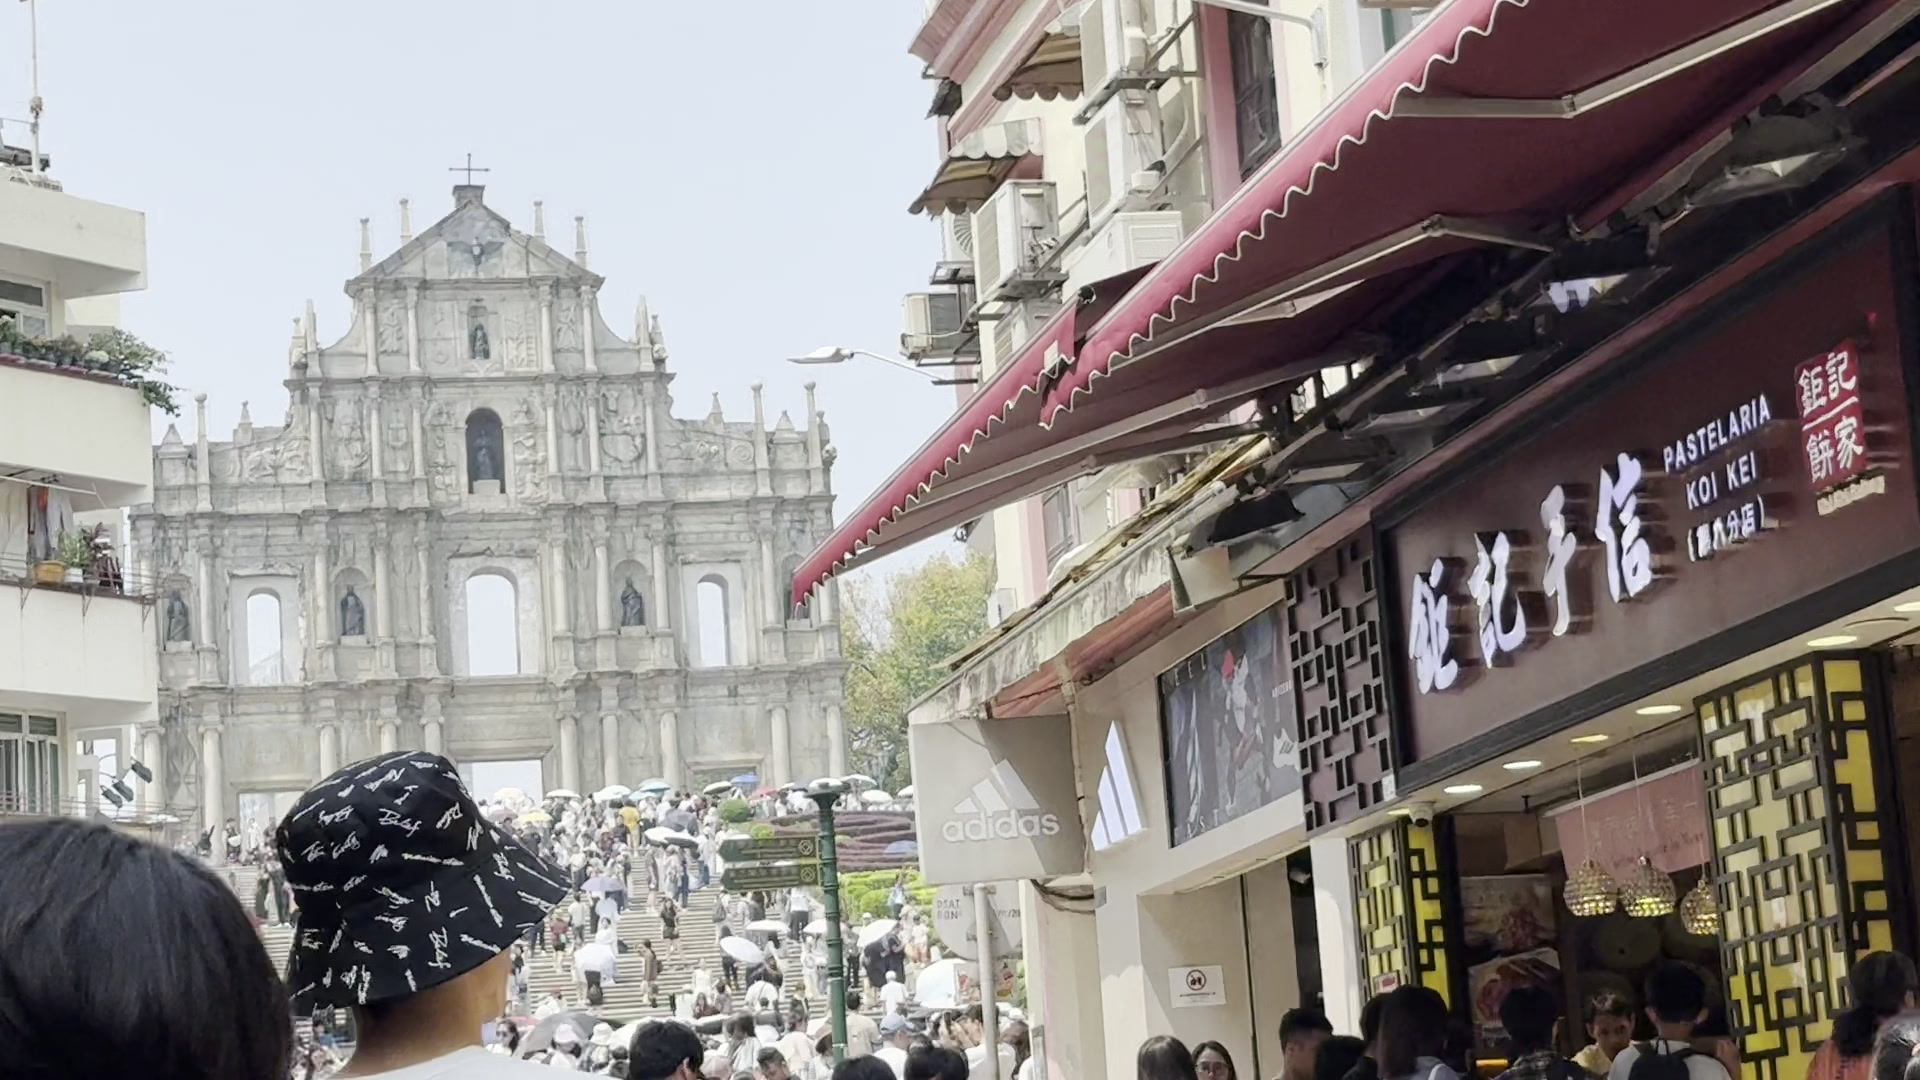
\includegraphics[width=0.82\linewidth]{fig11_street_to_ruins.jpg}
  \caption{Street view leading toward the Ruins of St. Paul's. The facade does not appear suddenly. It is gradually drawn out by shop signs, crowds, and the slope of the street.}
\end{figure}

The Ruins of St. Paul's is one of Macau's most recognisable heritage symbols. Visitors walked toward the facade, stopped in the square, looked up, and took photos. The steps and square made frontal viewing easy. MacCannell's (1973) staged authenticity helps explain what was happening: the heritage remains in place, but the square, the steps, and the photo positions also arrange it for visitors. The stone is four hundred years old. The posing is now.

Bilingual street signs offered another way of reading history. A sign guides movement, but it also places Chinese, Portuguese, historical naming, and the street scene together on one surface. Scollon and Scollon (2003) argue that signs should be read in their specific locations. Macau's blue-and-white tile signs matter because they combine two languages and sit inside old buildings, lanes, and tourist routes. One place, more than one historical system.

\begin{figure}[H]
  \centering
  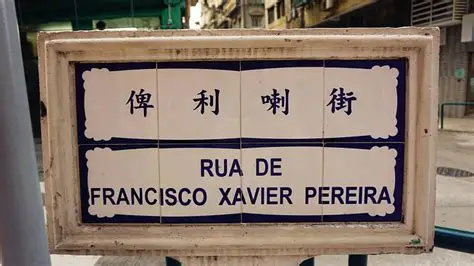
\includegraphics[width=0.72\linewidth]{fig05_bilingual_tile_street.png}
  \caption{Blue-and-white tile street sign for ``俾利喇街.'' The Portuguese historical name and Chinese street name appear on the same sign, turning the street name into an everyday historical text.}
\end{figure}

\begin{figure}[H]
  \centering
  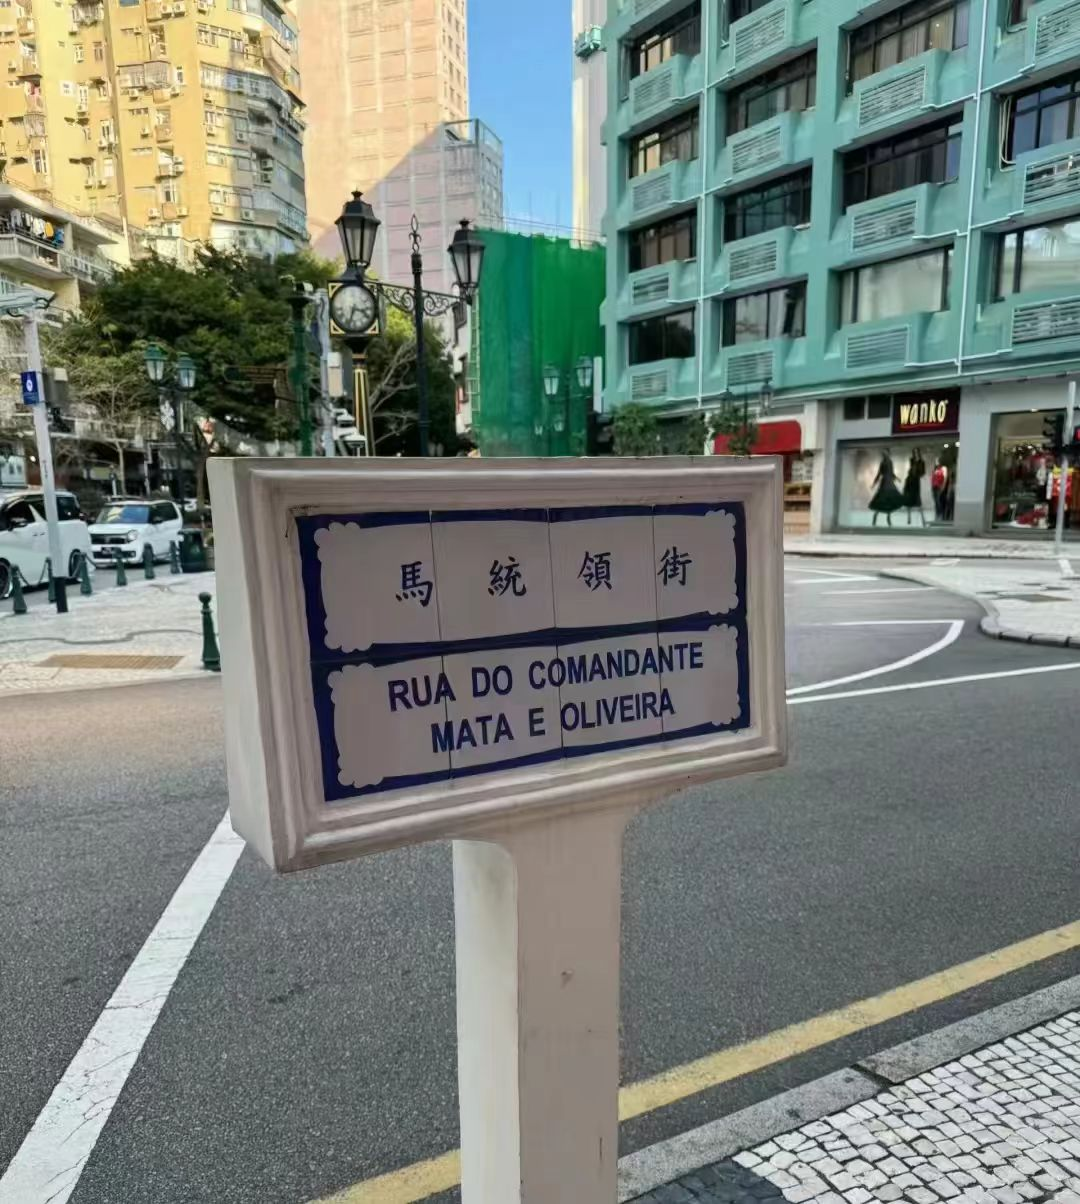
\includegraphics[width=0.72\linewidth]{fig06_bilingual_street_sign.jpg}
  \caption{Street sign for ``馬統領街.'' The Chinese and Portuguese names keep more than one layer of urban memory in the street.}
\end{figure}

Mount Fortress and the surrounding slopes made this bodily dimension even clearer. The uphill walk to the viewing platform, past stone walls and through narrow gates, turned history from a visual object into a physical one. Standing on the platform and looking over the modern city, the observer views present-day Macau from a position linked to the past. The historic area moved us away from the role of consumer and toward the role of viewer and reader.

\begin{figure}[H]
  \centering
  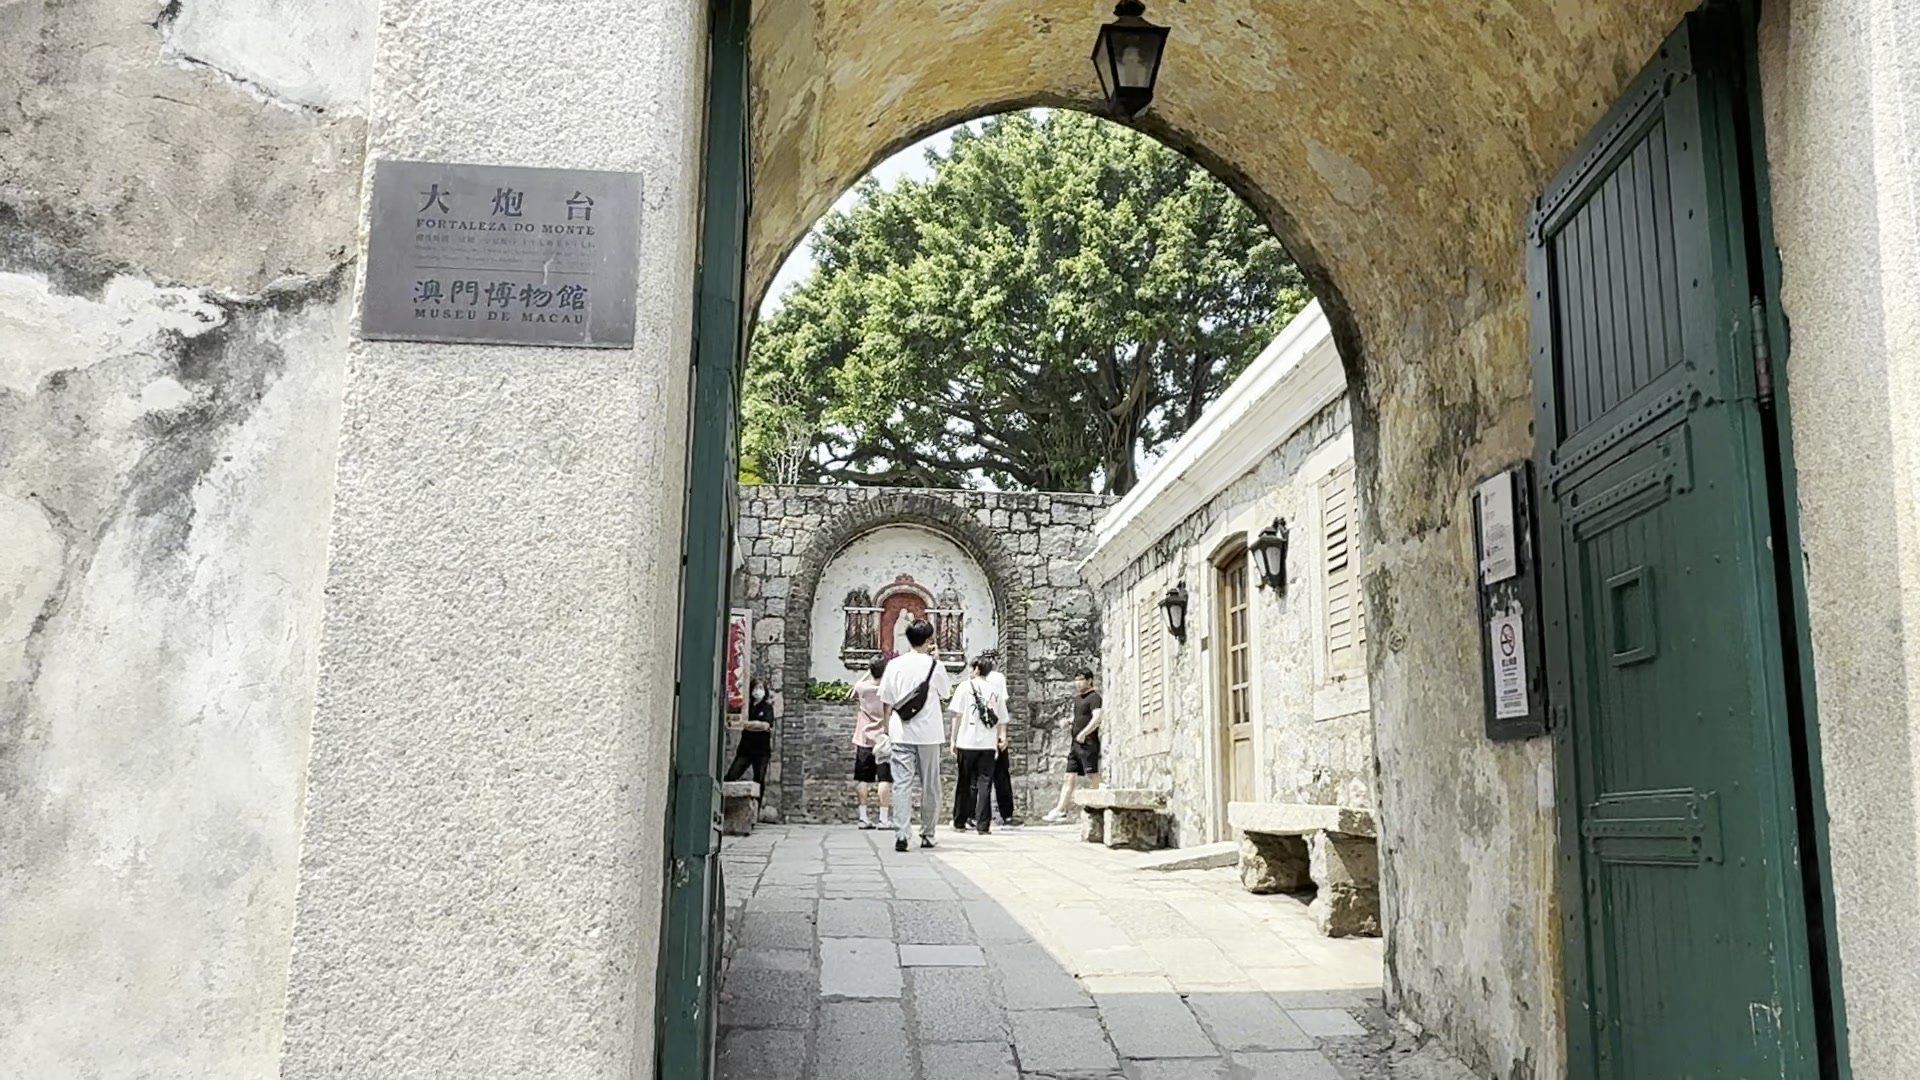
\includegraphics[width=0.82\linewidth]{fig12_fort_gate_path.jpg}
  \caption{Stone gate and path leading to Mount Fortress. The slope, stone wall, and entrance require the visitor to walk through heritage rather than only view it from a distance.}
\end{figure}

\subsection{Spectacle Macau}

After reaching Cotai, the cultural system shifted again. Hotel clusters, the Venetian, the Parisian, and the NBA-themed space did not tell a Chinese-Portuguese history. They placed European landmarks, casino hotels, and sports branding into one consumption route. Intercultural communication here was closer to global entertainment than to local heritage.

\begin{figure}[H]
  \centering
  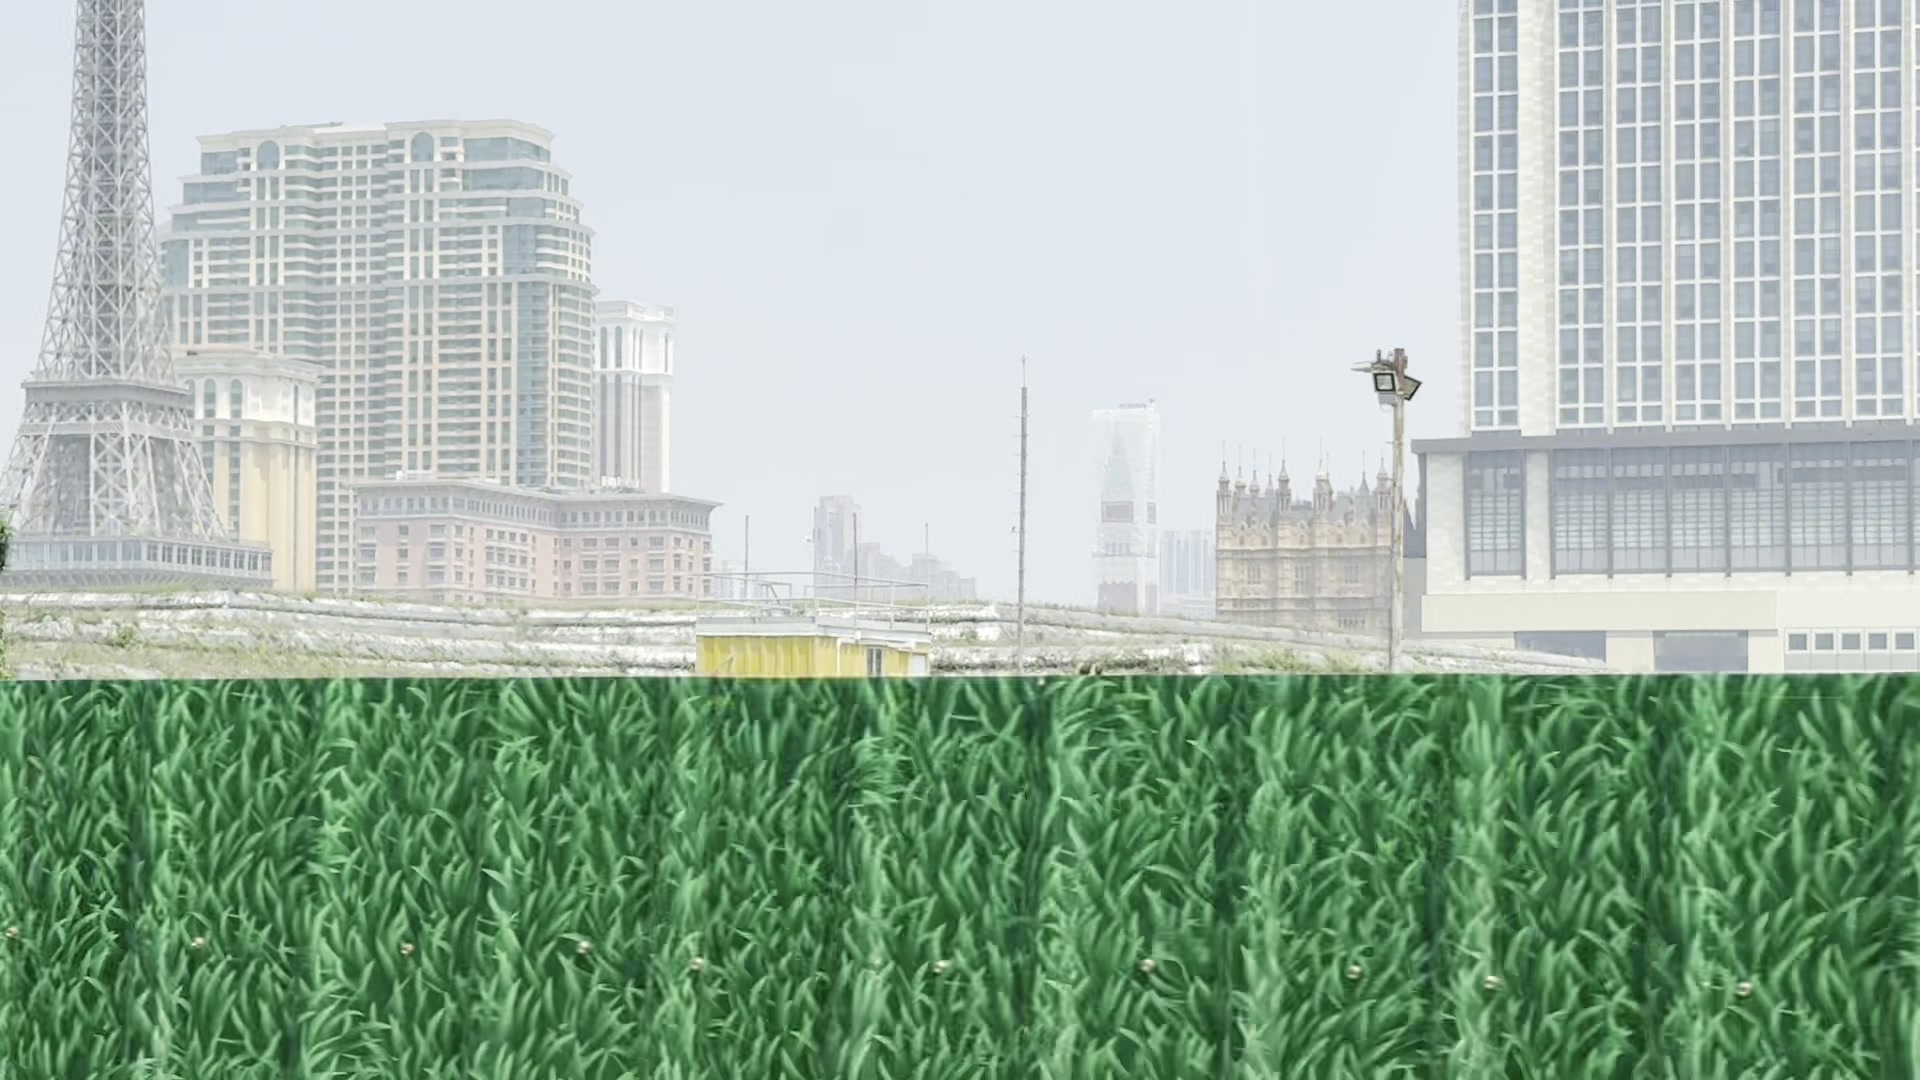
\includegraphics[width=0.82\linewidth]{fig07_cotai_parisian_window.jpg}
  \caption{Cotai hotel cluster and themed architecture seen from a vehicle window. Reproduced landmarks, hotels, and roads appear together in a moving view.}
\end{figure}

The Venetian is a designed European imagination inside Macau. Indoor ceilings painted like sky, murals, and classical-style decoration create an environment for shopping, photography, and lingering. Calling it ``fake Europe'' would miss the point. The sources are different from the Ruins of St. Paul's: one draws on historical layers and heritage narratives, the other on deliberate design and immersion. Both produce experience, but from different materials.

\begin{figure}[H]
  \centering
  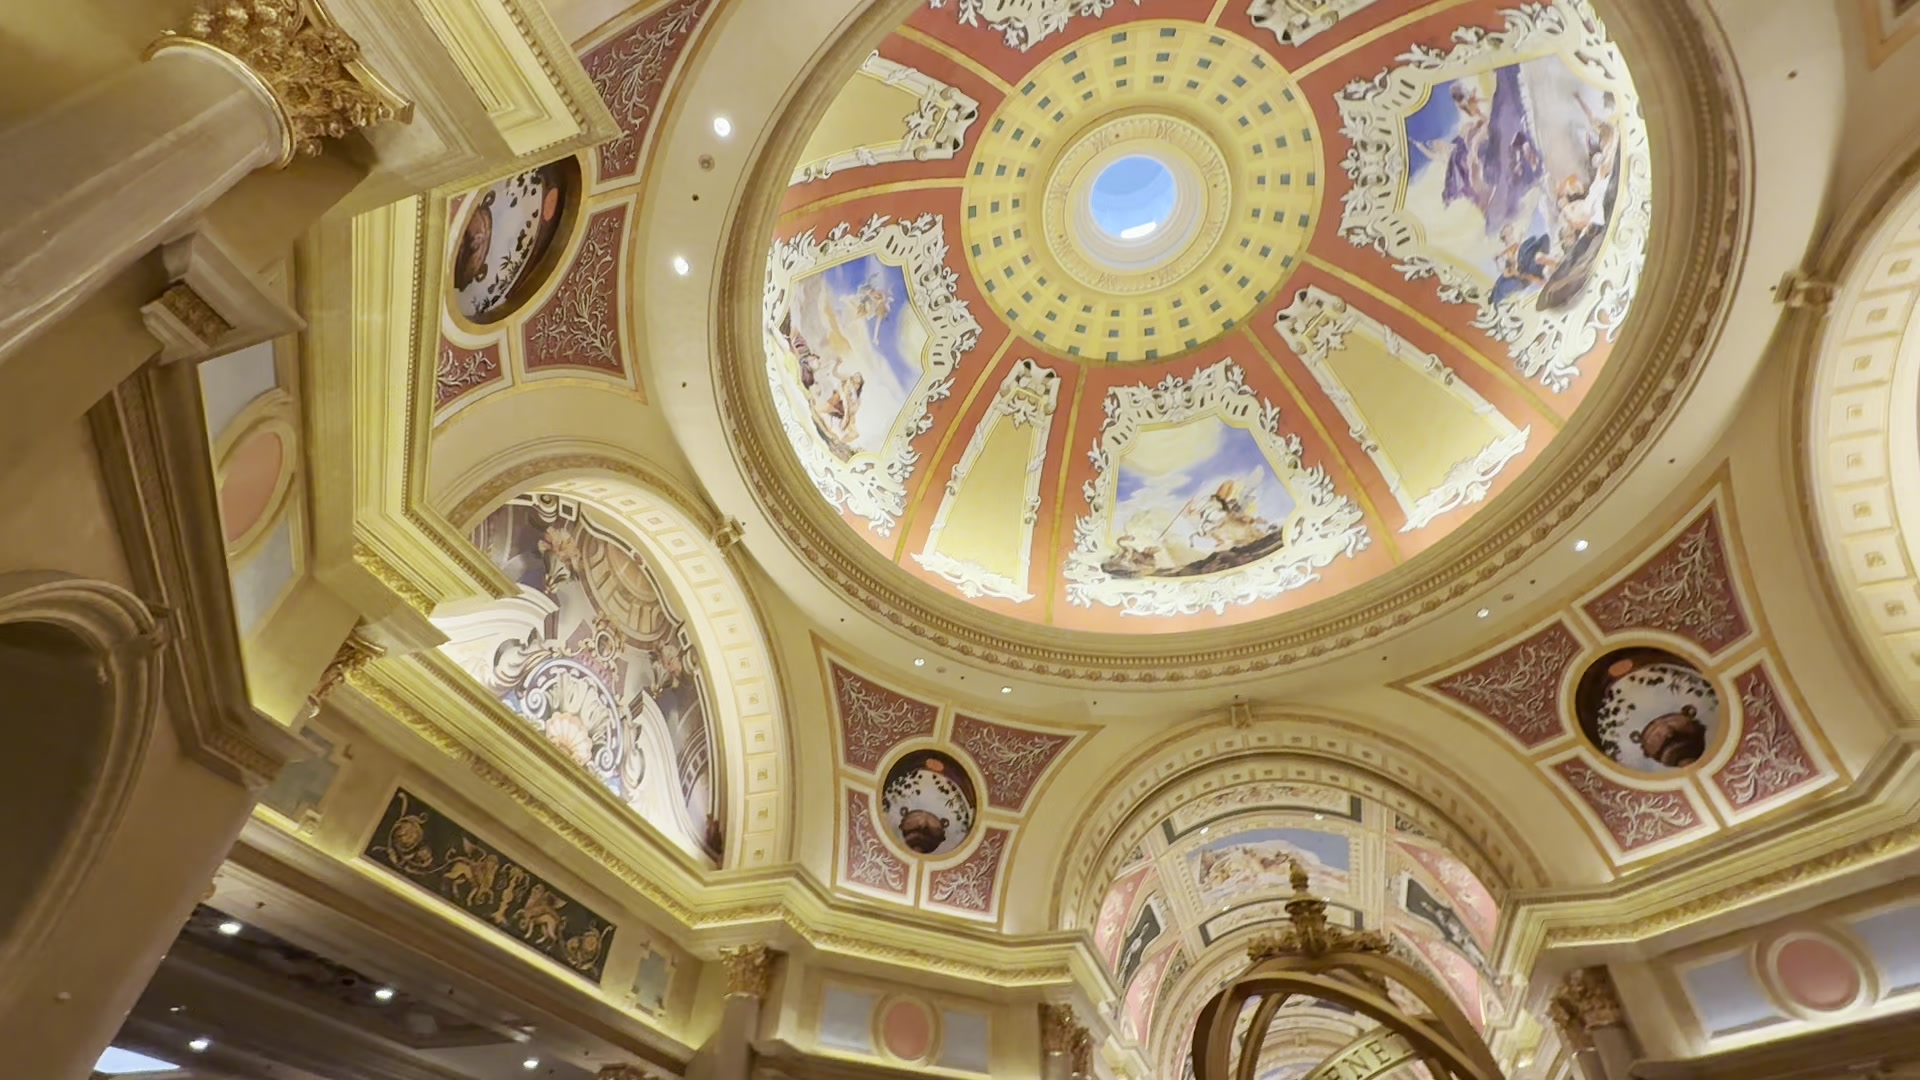
\includegraphics[width=0.82\linewidth]{fig8_venetian_dome.jpg}
  \caption{Interior dome in the Venetian. Upward viewing, murals, and classical-style decoration place a European imagination inside a shopping complex.}
\end{figure}

The wayfinding system matters too. The Cotai complex works as a consumption route more than as a single attraction. Casinos, hotels, restaurants, and themed buildings are connected through one directional system. These signs tell visitors where to go, but they also guide bodies toward the next scene of spending.

\begin{figure}[H]
  \centering
  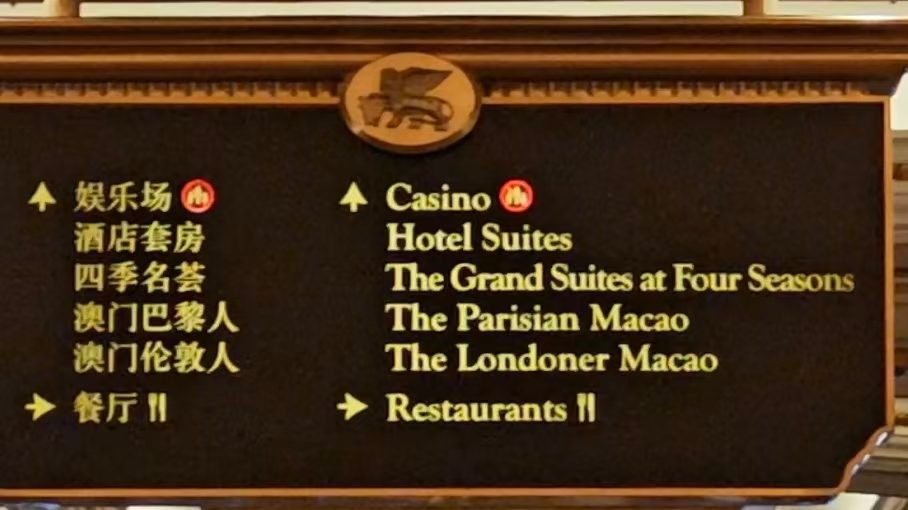
\includegraphics[width=0.82\linewidth]{fig08_wayfinding_casino.jpg}
  \caption{Casino and hotel wayfinding. Accommodation, gaming, dining, and shopping are connected by one directional system.}
\end{figure}

The NBA-themed space turned global popular culture into something visitors could touch and play with. American sports culture was not explained through text panels. It entered through jerseys on racks, court design, shooting movements, and a scoring screen. Wang's (1999) discussion of existential authenticity fits: visitors may not know the full history of American basketball, but the feeling of participation is real enough when the ball goes through the hoop.

\begin{figure}[H]
  \centering
  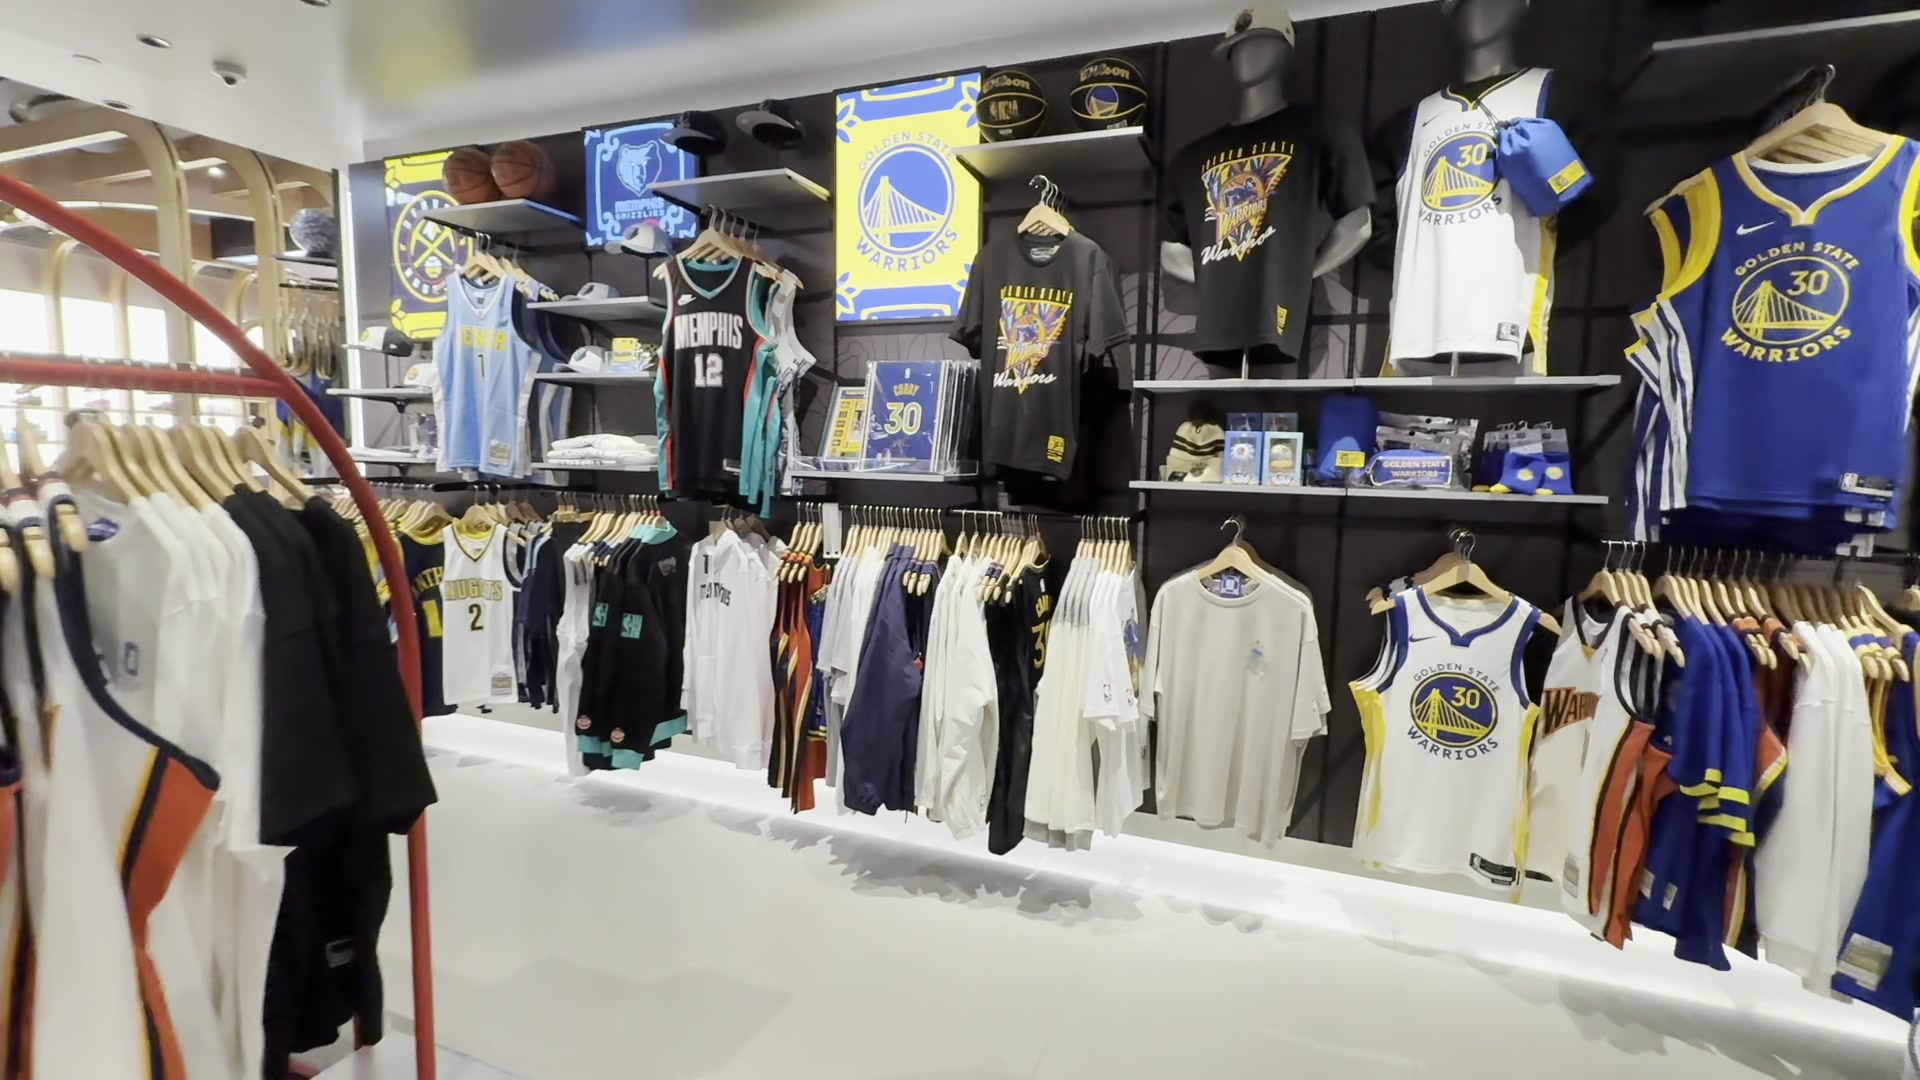
\includegraphics[width=0.82\linewidth]{fig10_nba_merchandise.jpg}
  \caption{Jerseys and merchandise in the NBA-themed space. Global sports culture first appears as products, team logos, and collectibles.}
\end{figure}

\begin{figure}[H]
  \centering
  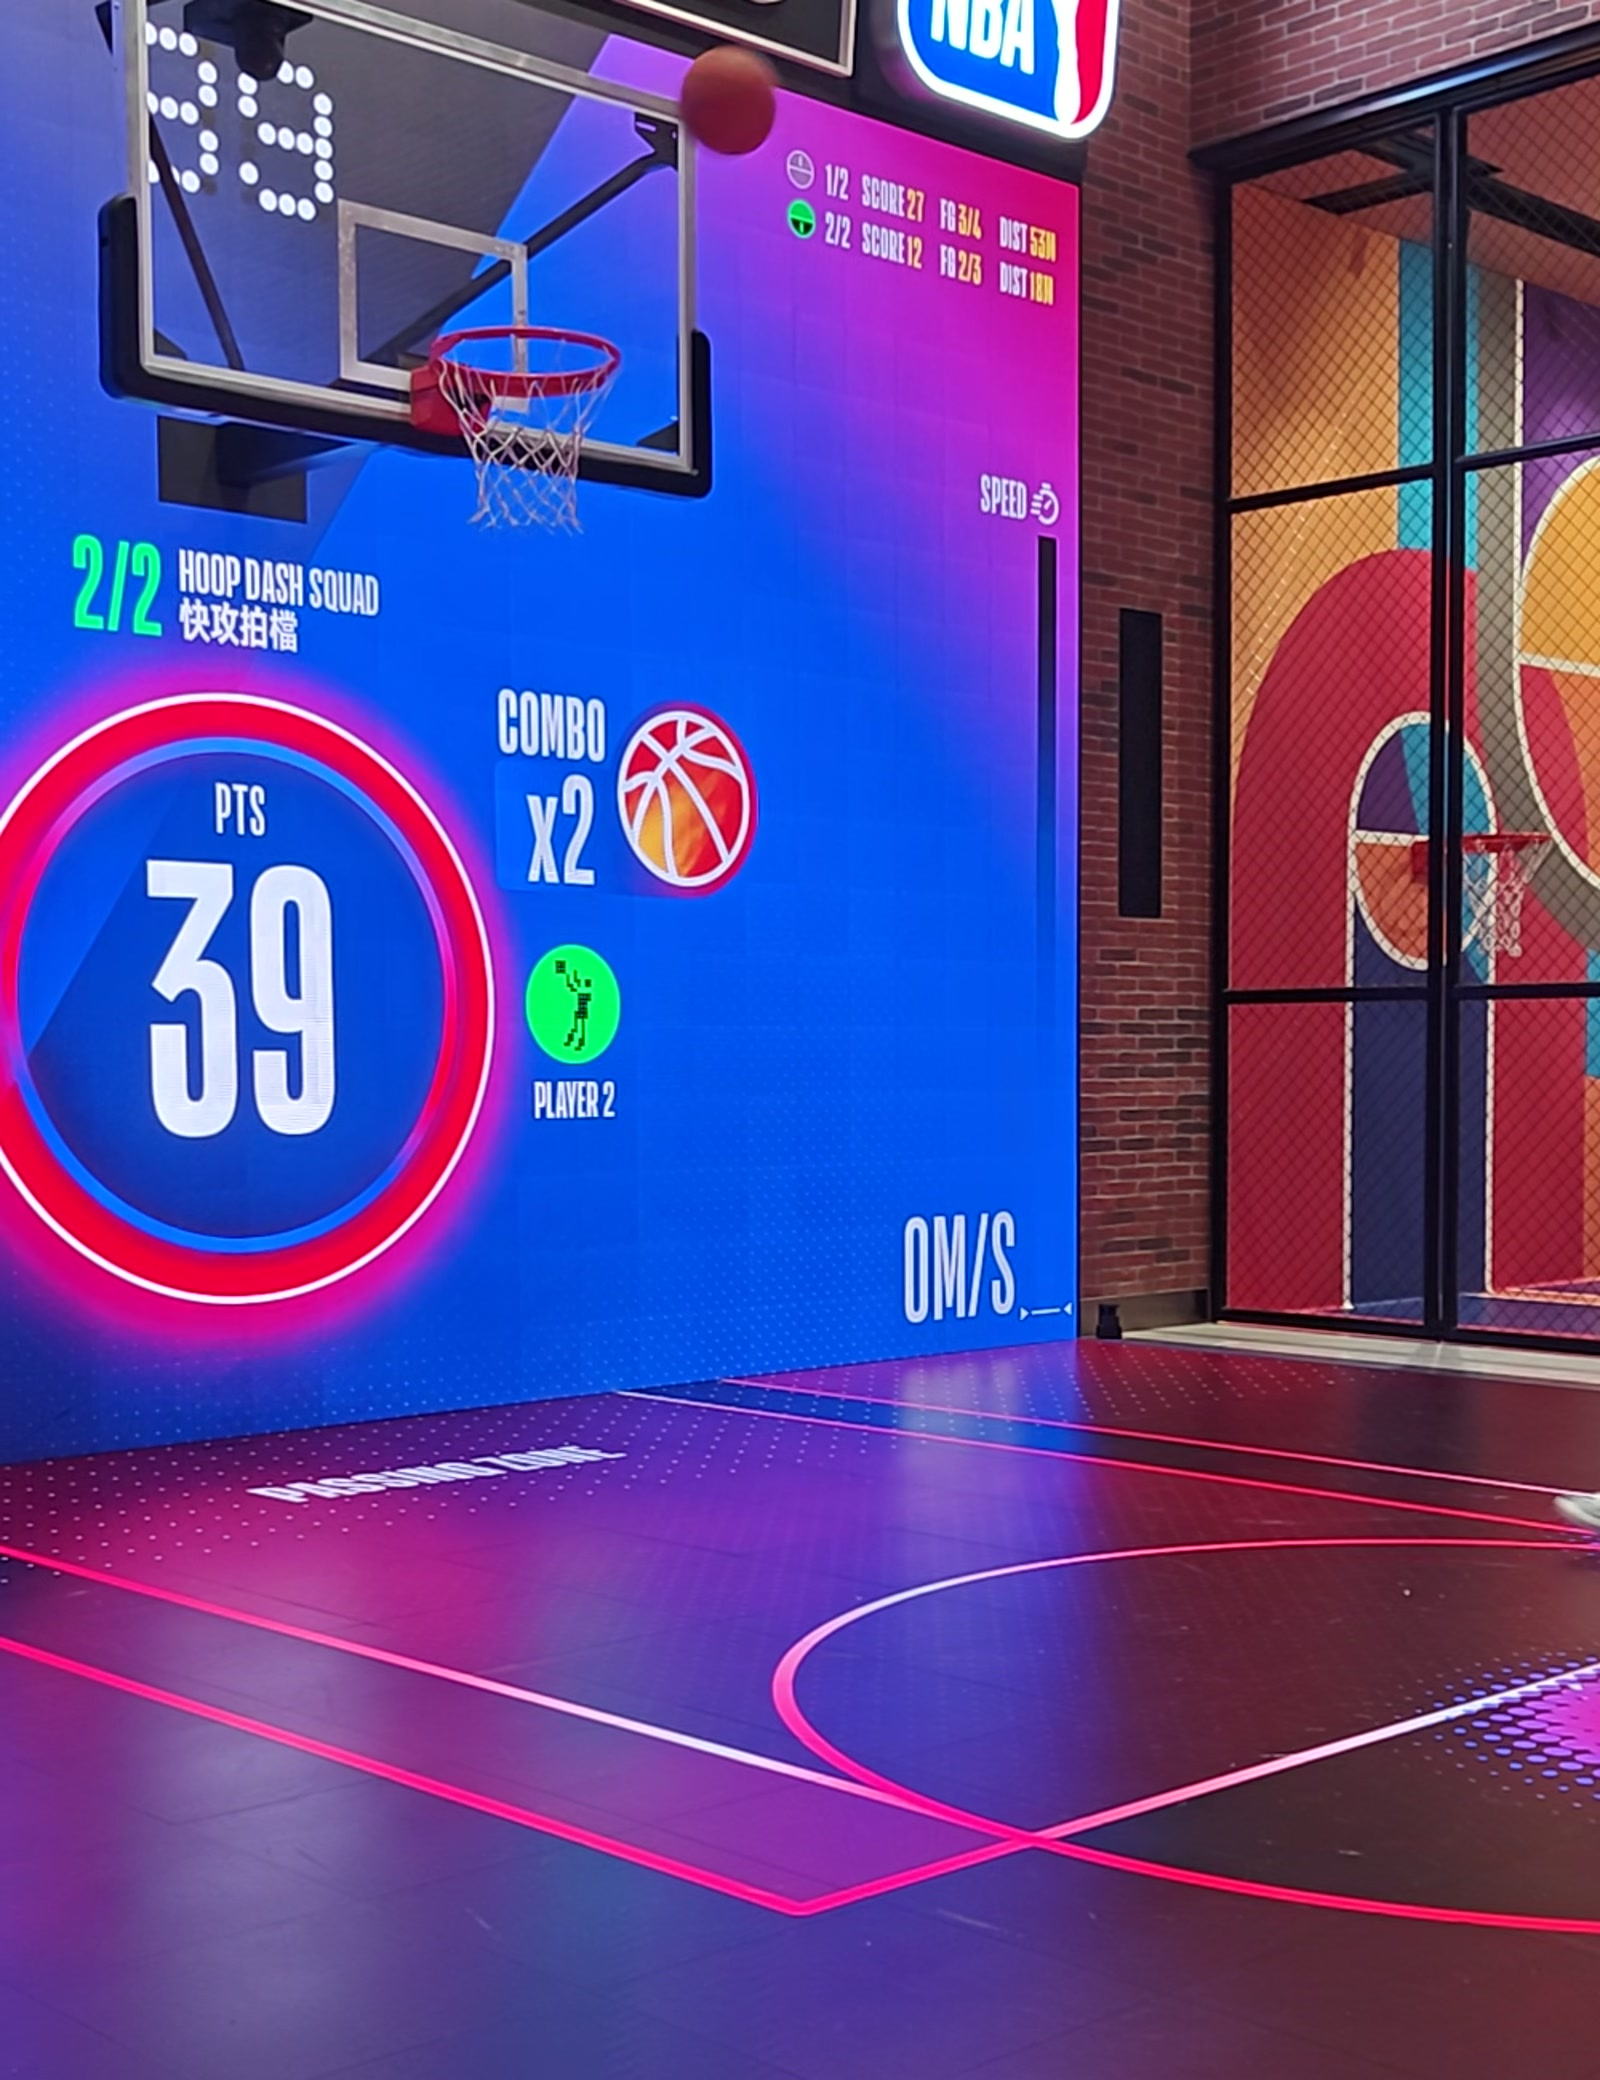
\includegraphics[width=0.82\linewidth]{fig7_nba.jpg}
  \caption{NBA shooting interaction area. Hoops, a scoring screen, and shooting movements turn sports culture into on-site participation.}
\end{figure}

\subsection{Transit Macau}

Transit spaces are easy to skip in a field trip report. Buses, shuttle vehicles, bridges, windows, and return carriages seem to connect destinations, nothing more. But they also made different versions of Macau appear one after another. Transit spaces did not display culture in the way that heritage sites or themed hotels did. They showed crowds, rhythm, and urban layers in everyday movement.

\begin{figure}[H]
  \centering
  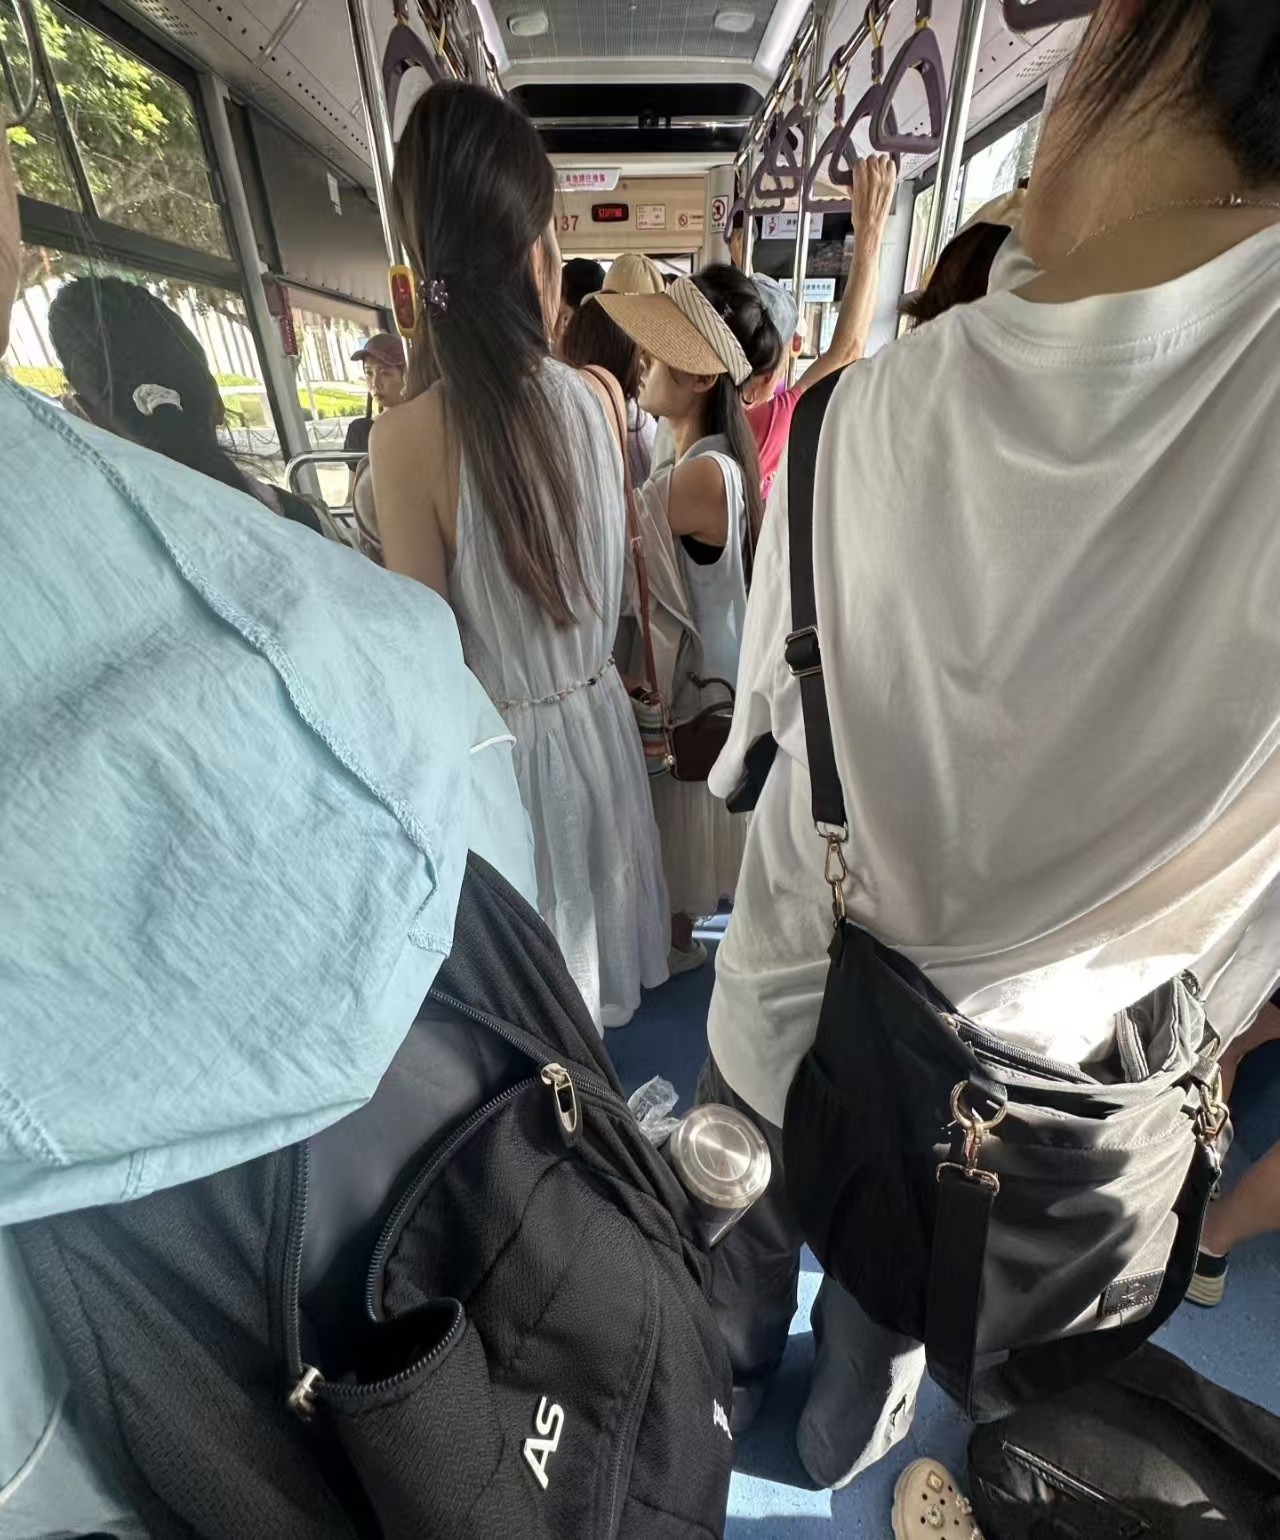
\includegraphics[width=0.82\linewidth]{fig10_bus_interior.jpg}
  \caption{Crowded bus interior. Handrails, standing bodies, and vehicle density show the order of movement inside transport space.}
\end{figure}

\begin{figure}[H]
  \centering
  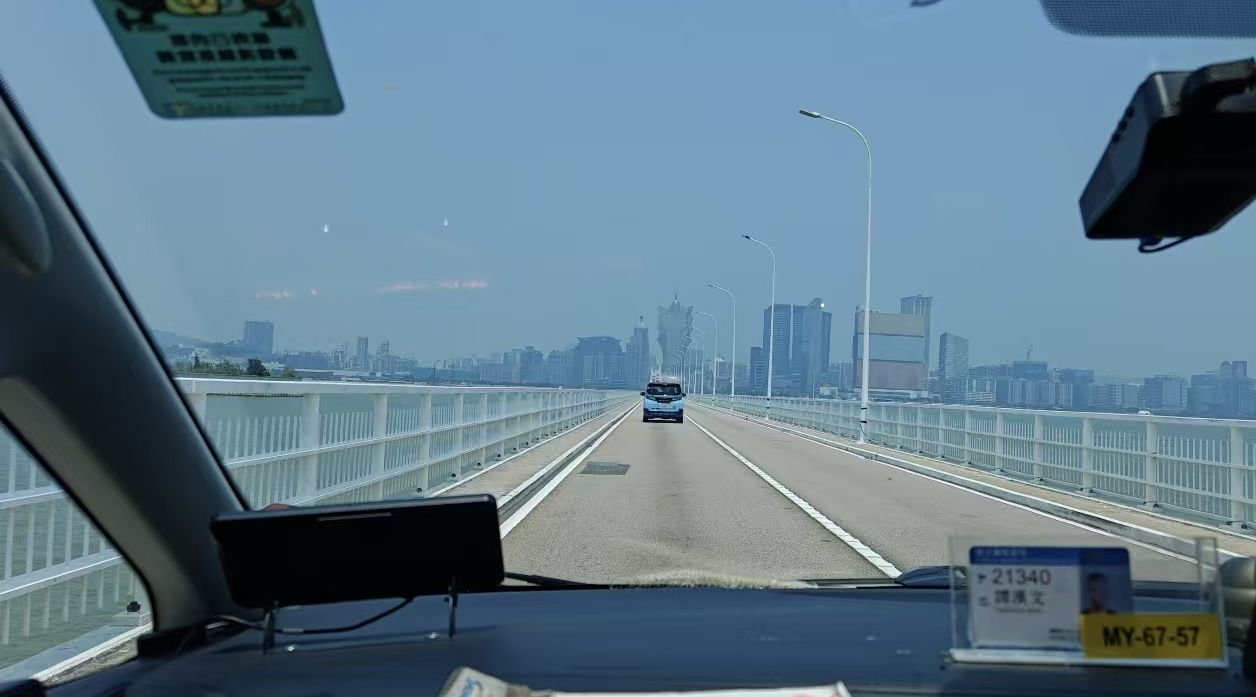
\includegraphics[width=0.82\linewidth]{fig12_vehicle_bridge.jpg}
  \caption{Bridge movement seen from inside a vehicle. The windshield, road, bridge, and distant skyline limit the observer to a window view.}
\end{figure}

Transit space shows that intercultural experience in Macau happens between destinations as well as at them. de Certeau (1984) and Pink (2009) both remind us not to treat movement as empty time. Role switching happens on these routes. The bus window, the bridge, the crowded seat: these are where one Macau gives way to the next.

\section{Discussion}

\subsection{Beyond fusion}

Chinese-Western fusion is a reasonable starting point for understanding Macau, but it falls short as a final explanation. It accounts for Chinese-Portuguese history, bilingual street names, and Portuguese-style lanes. It struggles with commercial streets, Cotai entertainment complexes, NBA-themed space, and transit. When fusion is used as the only label, different cultural elements are pushed into one static frame.

Our route suggests a different reading. Macau appeared as a sequence of spatial shifts, each with its own logic. The border imposed boundary and order. Then commercial streets pulled us into consumption and the historic area slowed us into heritage viewing, before Cotai swept us into global entertainment and the bus returned us to everyday urban movement. Each shift changed how we acted and what we noticed.

This reading does not deny Macau's Chinese-Portuguese history. Because that history matters, it needs to be separated from other cultural systems. Cultural sensitivity cannot stop at the observation that ``many cultures are present.'' It needs to ask who is guided into the city, who is invited to consume, who is positioned to view history, and who participates in global entertainment through interaction. These questions explain the field materials better than asking whether Macau is a fusion city.

\subsection{The route changes the question}

If we analyse each site by itself, Macau breaks into unrelated tourist spots: the border is transport, the Ruins of St. Paul's is heritage, the commercial street is consumption, the Venetian is entertainment, the bus is movement. Once these places are connected through a route, the question changes. The transitions between places become part of the analysis.

The transitions also changed our position. At the border, institutional procedures managed our entry. By the time we reached the food streets, those procedures had been replaced by the pull of commerce and crowds. Later, standing in front of the Ruins of St. Paul's or inside the Venetian, the questions changed again, from what to buy to what to look at to how to play. Back on the bus, we watched the city overlap through the window.

The route also reminds us that we were not outside Macau giving a neutral explanation. We were repeatedly positioned by the systems around us. The question shifts from what culture Macau ``is'' to how people are arranged to experience culture in different spaces.

\subsection{From signs to bodies}

Intercultural communication is more than language translation. Chinese-Portuguese street signs and NBA English interfaces shape place identity, and so do the non-verbal cues that filled the spaces between them. Border corridors channel bodies without words. Steps and squares at the Ruins of St. Paul's arrange viewing through physical placement. Ceilings and lighting in the Venetian create immersion without a sentence being spoken. Hoops and scoring screens at the NBA court turn culture into a game of shooting. Even the bus window frames what can and cannot be seen.

This report therefore looks at two levels at once: what a space says, and what it does to bodies and actions. Landry and Bourhis (1997) help explain how multilingual signs shape place identity. Scollon and Scollon (2003) move signs back into their concrete locations. Hall (1959) reminds us that spatial order is already a form of non-verbal communication. Macau's intercultural meaning is formed between written signs, bodily order, and sensory experience.

\subsection{Misreading and interpretation}

The course value of this report lies partly in correcting several likely misreadings. Calling Macau simply a Chinese-Western fusion city hides differences between the border, commercial streets, historic area, and Cotai. Treating commercialisation as a weakening of history misses how commercial streets also circulate heritage landmarks through taste and crowds. Calling the Venetian ``fake Europe'' ignores how it produces experience through design and participation inside Macau's tourism economy. One more limit matters: we cannot infer residents' or tourists' subjective attitudes directly from crowded photos, because this study did not include formal interviews.

From a cultural relativist perspective, intercultural understanding should not rush to label a space as real or unreal. A better approach is to ask how it works in its setting, whom it serves, and what simplifications it may produce. When quick explanations such as ``fusion'' or ``fake Europe'' are not enough, the researcher has to return to concrete spaces, routes, and bodily experience. That process of revision is part of reflective intercultural communication.

\section{Conclusion}

Macau's intercultural character does not sit in one place. It shifts as the route moves. We entered as managed subjects at the border, became buyers on the food streets, slowed into viewers at the old stone facades, and then sped up again as participants in themed entertainment before the bus returned us to watching the city scroll past.

Chinese-Western fusion is real in Macau. Chinese-Portuguese writing, Portuguese-style architecture, and World Heritage sites are there, physically present on the streets. But queues, wayfinding signs, vehicle windows, shop displays, painted ceilings, and bodily movements also shape cultural experience, and fusion alone cannot account for them.

The report has limits. Without formal interviews, it cannot represent the subjective voices of residents, tourists, or workers. The route is limited, so it cannot cover all Macau neighbourhoods. Sound and sensory observations were not collected through a systematic audio study and remain supplementary field notes. Future research could add interviews with residents and tourists, compare different routes, or record linguistic landscapes and transit spaces more systematically.

For cross-cultural communication, the field trip gives one main reminder: do not label a city too quickly. Entering specific spaces and watching how people move, view, consume, and participate allows a more careful understanding of how culture is seen, used, and reinterpreted in the city.

\section*{References}
\addcontentsline{toc}{section}{References}

\noindent\hangindent=1.5em\hangafter=1
Chu, C. L. (2015). Spectacular Macau: Visioning futures for a World Heritage city. \textit{Geoforum, 65}, 440--450. \url{https://doi.org/10.1016/j.geoforum.2015.06.009}

\noindent\hangindent=1.5em\hangafter=1
Chung, T. (2009). Valuing heritage in Macau: On contexts and processes of urban conservation. \textit{Journal of Current Chinese Affairs, 38}(1), 129--160. \url{https://doi.org/10.1177/186810260903800107}

\noindent\hangindent=1.5em\hangafter=1
de Certeau, M. (1984). \textit{The practice of everyday life} (S. Rendall, Trans.). University of California Press.

\noindent\hangindent=1.5em\hangafter=1
Edensor, T. (2000). Staging tourism: Tourists as performers. \textit{Annals of Tourism Research, 27}(2), 322--344. \url{https://doi.org/10.1016/S0160-7383(99)00082-1}

\noindent\hangindent=1.5em\hangafter=1
Hall, E. T. (1959). \textit{The silent language}. Doubleday.

\noindent\hangindent=1.5em\hangafter=1
Landry, R., \& Bourhis, R. Y. (1997). Linguistic landscape and ethnolinguistic vitality: An empirical study. \textit{Journal of Language and Social Psychology, 16}(1), 23--49. \url{https://doi.org/10.1177/0261927X970161002}

\noindent\hangindent=1.5em\hangafter=1
Lefebvre, H. (1991). \textit{The production of space} (D. Nicholson-Smith, Trans.). Blackwell.

\noindent\hangindent=1.5em\hangafter=1
Ma, Q., \& Mu, C. (2023). Multilingual practices of translation in Macao's linguistic landscape: A case study of Rua do Campo. \textit{Cadernos de Tradução, 43}(1), 1--22. \url{https://doi.org/10.5007/2175-7968.2023.e90223}

\noindent\hangindent=1.5em\hangafter=1
MacCannell, D. (1973). Staged authenticity: Arrangements of social space in tourist settings. \textit{American Journal of Sociology, 79}(3), 589--603. \url{https://doi.org/10.1086/225585}

\noindent\hangindent=1.5em\hangafter=1
Pink, S. (2009). \textit{Doing sensory ethnography}. SAGE.

\noindent\hangindent=1.5em\hangafter=1
Scollon, R., \& Scollon, S. W. (2003). \textit{Discourses in place: Language in the material world}. Routledge.

\noindent\hangindent=1.5em\hangafter=1
UNESCO World Heritage Centre. (n.d.). \textit{Historic Centre of Macao}. Retrieved May 5, 2026, from \url{https://whc.unesco.org/en/list/1110/}

\noindent\hangindent=1.5em\hangafter=1
Urry, J., \& Larsen, J. (2011). \textit{The tourist gaze 3.0}. SAGE.

\noindent\hangindent=1.5em\hangafter=1
Wang, N. (1999). Rethinking authenticity in tourism experience. \textit{Annals of Tourism Research, 26}(2), 349--370. \url{https://doi.org/10.1016/S0160-7383(98)00103-0}

\noindent\hangindent=1.5em\hangafter=1
Yan, X. (2019). Language choices in the linguistic landscape of Macao. \textit{Journal of Multilingual and Multicultural Development, 40}(3), 198--217. \url{https://doi.org/10.1080/01434632.2018.1498853}

\appendix

\section{Field trip route table}

\begin{table}[H]
\centering
\caption{Field trip route, observer roles and space types}
\begin{tabular}{>{\raggedright\arraybackslash}p{0.18\linewidth}>{\raggedright\arraybackslash}p{0.23\linewidth}>{\raggedright\arraybackslash}p{0.25\linewidth}>{\raggedright\arraybackslash}p{0.22\linewidth}}
\toprule
Route stage & Main spaces & Observer role & Main mechanisms \\
\midrule
Entering Macau & Border, queue area, transport connections & Entrant & Queuing, wayfinding, immigration, window views \\
Commercial streets & Food streets, souvenir streets, signs, crowds & Consumer & Products, linguistic landscape, crowded streets \\
Historic area & Ruins of St. Paul's, church spaces, Mount Fortress, street signs & Viewer and reader & Walking, photography, bilingual signs, overlooking the city \\
Cotai spectacle & Venetian, Parisian, casino spaces, NBA-themed space & Global entertainment participant & Themed design, wayfinding, shopping, interactive games \\
Transit spaces & Buses, bridges, return vehicles & Moving observer & Windows, crowding, overlapping urban layers \\
\bottomrule
\end{tabular}
\end{table}

\section{Selected media inventory}

\begin{longtable}{>{\raggedright\arraybackslash}p{0.1\linewidth}>{\raggedright\arraybackslash}p{0.12\linewidth}>{\raggedright\arraybackslash}p{0.28\linewidth}>{\raggedright\arraybackslash}p{0.38\linewidth}}
\caption{Selected images and their analytical functions}\\
\toprule
Figure & File & Scene & Analytical function \\
\midrule
\endfirsthead
\toprule
Figure & File & Scene & Analytical function \\
\midrule
\endhead
Fig. 1 & fig01 & Transport wayfinding toward Macau & Shows that intercultural experience begins with entry, signs and movement. \\
Fig. 2 & fig02 & Commercial street crowds near the Ruins of St. Paul's & Shows how crowded streets change the rhythm of heritage viewing. \\
Fig. 3 & fig03 & Street bakery and snack stall & Shows how taste, purchase and pausing become bodily experience. \\
Fig. 4 & fig04 & Street leading to the Ruins of St. Paul's & Shows how heritage viewing is shaped by street movement and commerce. \\
Fig. 5 & fig05 & Blue-and-white tile street sign & Shows how bilingual street signs preserve urban memory. \\
Fig. 6 & fig06 & ``馬統領街'' street sign & Shows how street names become historical texts in everyday space. \\
Fig. 7 & fig07 & Entrance path to Mount Fortress & Shows how heritage becomes a walking experience. \\
Fig. 8 & fig08 & Cotai window view & Shows how themed architecture enters the urban imagination. \\
Fig. 9 & fig09 & Interior dome in the Venetian & Shows how European imagery is designed as immersive experience. \\
Fig. 10 & fig10 & Casino and hotel wayfinding & Shows how wayfinding organises Cotai's consumption route. \\
Fig. 11 & fig11 & NBA merchandise display & Shows how global sports culture becomes commodity. \\
Fig. 12 & fig12 & NBA shooting interaction area & Shows how sports culture becomes participatory entertainment. \\
Fig. 13 & fig13 & Bus interior & Shows the movement order inside transit space. \\
Fig. 14 & fig14 & Bridge view from inside a vehicle & Shows how vehicle windows frame Macau in motion. \\
\bottomrule
\end{longtable}

\section{Course ILO and rubric alignment}

\begin{table}[H]
\small
\centering
\caption{Alignment between course ILOs and report content}
\begin{tabular}{>{\raggedright\arraybackslash}p{0.14\linewidth}>{\raggedright\arraybackslash}p{0.42\linewidth}>{\raggedright\arraybackslash}p{0.32\linewidth}}
\toprule
Course goal & Report alignment & Main sections \\
\midrule
ILO\#1 & Route entry and role switching show the spatial relation between observer and other & Introduction, Findings, Discussion 5.2 \\
ILO\#2 & The report avoids reducing Macau to a single fusion label and distinguishes different cultural logics & Introduction, Discussion 5.1 \\
ILO\#3 & The report analyses verbal and non-verbal communication in street signs, shop signs, wayfinding, queues, windows and interactive facilities & Framework, Findings, Discussion 5.3 \\
ILO\#4 & The route is used to build a culturally aware fieldwork narrative rather than a list of tourist spots & Methodology, Discussion 5.2 \\
ILO\#5 & The report identifies and corrects interpretive misreadings such as ``fake Europe'' and ``commercialisation weakens history'' & Discussion 5.4, Conclusion \\
\bottomrule
\end{tabular}
\end{table}

\end{document}
